\title{MIET Project Template}
\author{Team Compile}
\date{August 2024}

\documentclass[12pt]{report}
\usepackage[utf8]{inputenc}

% Packages for mathematical formulas, graphics, and layout
\usepackage{amsmath, amsfonts, amssymb}
\usepackage{graphicx, caption, subcaption}
\usepackage{longtable, multirow, tabularx}
\usepackage[a4paper,width=160mm,top=25mm,bottom=25mm]{geometry}

% Listings package for pseudocode and code formatting
\usepackage{listings}
\usepackage{xcolor}


%additional packages
\usepackage{verbatim}
\usepackage{cite}
\usepackage{graphicx}
\usepackage{listings}
\usepackage{xcolor}
\usepackage{minted}
\usepackage{amsmath}
\usepackage{lipsum}
\usepackage{graphicx}
\usepackage{caption}
\usepackage{subcaption}
\usepackage{longtable}
\graphicspath{{figures/}}
\usepackage[a4paper,width=160mm,top=25mm,bottom=25mm]{geometry}
\usepackage{titlesec}
\linespread{1.2}
\usepackage{subcaption}
\usepackage{schemabloc,tikz}
\usepackage{amsfonts,epsfig,cite,array,multirow,graphicx,amsmath,amsthm,ltablex,tabularx,setspace,arydshln,amssymb,multirow}
\usetikzlibrary{circuits, arrows}
\newtheorem{theorem}{Theorem}
\newtheorem{lemma}{Lemma}
\usepackage[utf8]{inputenc}
\usepackage{amsmath}
\usepackage{amsfonts}
\usepackage{amssymb}
\usepackage{bbm}
\usepackage{mathtools}
\usepackage{textcomp}
\usepackage{stackengine}
\usepackage{booktabs}
\usepackage{longtable}
\usepackage{multirow}
\usepackage{graphicx}
\usepackage{subcaption}
\usepackage{ragged2e}
\usepackage{biblatex}
%\usepackage[backend=biber,style=alphabetic,sorting=ynt]{biblatex}
\addbibresource{references.bib}
% hyperlinks
\usepackage{hyperref} 
\hypersetup{ colorlinks, citecolor=blue, filecolor=black, linkcolor=black, urlcolor=blue } 

\def\mytitle{Talent Trail}
\def\myname{\textbf{Atul Kumar[2021a1r072]\\ \vspace{0.1cm} Akshat Amla [2021a1r064]\\ \vspace{0.1cm} Vivek Koul [2021a1r080]}\\}
\def\degree{Bachelor of Technology}
\def\mydegree{Computer Science \& Engineering}
\def\mysupervisor{Dr. Mehak Mengi \\ Assistant Professor, CSE}
\def\myrollno{2021A1RXX}
\def\mydep{Department of Computer Sciences and Engineering}
\addbibresource{references.bib}
\begin{document}

%Front Matter
\thispagestyle{empty}
\begin{center}
%\vspace*{0.3cm}
    { \Large {\bfseries {INFLUENCIFY- A platform for brand collaborations and co-creations} \par}
\vspace{0.5\baselineskip}

    {\textit{A major project report submitted in partial fulfillment for}\\
    \textit{the award of degree of}}\par
\vspace{0.1\baselineskip}

    {\Large \bf Bachelor of Engineering \par}
\vspace{0.1\baselineskip}

    {\textit{in} \par}
\vspace{0.1\baselineskip}

    {\Large \bf Computer Science and Engineering \par} 
% \vspace{\baselineskip}

    {\textit{by} \par}
% \vspace{\baselineskip}

    {{\Large \textbf{{Harpreet Kour [2021A1R042]}}} \par}
    {{\Large \textbf{{Shradha Sharma [2022A1L016]}}} \par}
   

\vspace{1\baselineskip}

    {\large Under the Supervision of \par}
% \vspace{0.3\baselineskip}

   
     {{\Large \bf Dr Rajneet Kaur Bijral} \par}
       {{\Large \bf Assistant Professor,CSE} \par}
    
\vspace{\baselineskip}

    {\begin{figure}[!h] 
	\centering
	
\includegraphics[width=0.5\linewidth]{Images/MIET_LOGO_AUTONOMOUS.png} 
     \end{figure}
    }
\vspace{0.2\baselineskip}

    {\large \MakeUppercase{\mydep} \par}
\vspace*{2ex}

    {\large \uppercase{Model Institute of Engineering and Technology} \par}
    \uppercase{{Jammu, J\&K, India}}\\
\vspace{0.3cm}

    {\large \textbf{Batch 2021-2025}\\}
\vspace{0.5cm}
\end{center}

 \pagenumbering{roman}
% \begin{certi}
    \begin{center}
 
        \vspace*{0.1cm}
        \large
        \begin{flushright}
        \text{ MIET\slash CSE\slash PR\slash ...\slash 2024-25 }
        \end{flushright}
        
    
\includegraphics[width=0.2\textwidth]{Images/miet_round_logo.png}\\
        \textbf{Model Institute of Engineering \& Technology, Jammu}
        
        \vspace{0.8cm}
        
        \large
        \textbf{Certificate}\\
        \vspace{0.5cm}
        
    \end{center}
% \end{certi}
\noindent
{\large This is to certify that this Major Project  entitled \textbf{INFLUENCIFY- A platform for brand collaborations and co-creations} is a bonafide work of \textbf{Harpreet Kour(2021A1R042), Shradha Sharma(2022A1l016)} submitted to the Model Institute of Engineering \& Technology, Jammu in partial fulfillment of the requirements for the award of the degree of "Bachelors of Technology" in Computer Science \& Engineering.}
\vspace{2cm}

\begin{table}[h]
\centering
\begin{tabular}{cp{2cm}p{2cm}c}
\hrulefill & & & \hrulefill \\
\large (Name and sign) & & & \large (Name and sign) \\
\large Guide & & & \large External Examiner \\
\end{tabular}
\end{table}

\centering \textbf{College Seal}\\
  \vspace{2cm}

\begin{table}[h]
\centering
\begin{tabular}{cp{2cm}p{2cm}c}
\hrulefill & & & \hrulefill  \\
\large (Name and sign) & & &\large (Name and sign) \\
\large Internal Examiner & &  & \large HOD,CSE \\
\end{tabular}
\end{table}

\vspace{1cm}
\noindent



\addcontentsline{toc}{chapter}{Certificate}
\newpage
    \begin{center}
    
        \vspace*{0.1cm}
        \large
       

        
        \vspace{0.8cm}
        
        \large
        \textbf{Certificate of Approval of Examiners}\\
        \vspace{0.5cm}
        
    \end{center}

    

{\large The Major Project report entitled  \textbf{INFLUENCIFY- A platform for brand collaborations and co-creations}  by \textbf{Harpreet Kour(2021A1R042), Shradha Sharma(2022A1l016)} is approved for the award of Bachelors of Technology Degree in \textbf{Computer Science \& Engineering}.} 

\vspace{2cm}

    

\begin{table}[h]
\begin{flushright}
\begin{tabular}{Y}
\hrulefill\\
\large Internal Examiner\\
\end{tabular}
\end{flushright}
\end{table}

\vspace{1cm}
\hfill
\begin{table}[h]
\begin{flushright}
\begin{tabular}{Y}
\hrulefill\\
\large External Examiner
\end{tabular}
\end{flushright}
\end{table}

\vspace{1cm}
\noindent


\begin{flushleft}
{\large Date:}\\
{\large Place: Jammu}
\end{flushleft}
\addcontentsline{toc}{chapter}{Certificate of Approval of Examiners}
\chapter*{Acknowledgment}
\begin{justify}
I take this opportunity to express my heartfelt gratitude to all those who have contributed directly or indirectly to the successful completion of my project, \textbf{“INFLUENCIFY- A platform for brand collaborations and co-creations
”} Their support, guidance, and encouragement have been instrumental in every step of this journey.  

First and foremost, I would like to extend my deepest gratitude to the \textbf{Dr. Navin M. Upadhyay,(HOD CSE)}, for their unwavering support and for providing the infrastructure and academic resources that enabled this project to take shape. My sincere thanks also go to the \textbf{External Examiner} and \textbf{Internal Examiner}, whose invaluable feedback, constructive criticism, and insights refined the outcomes of this project and ensured its alignment with the required standards. I am equally grateful to the \textbf{Tech Support Team}, whose technical assistance, troubleshooting expertise, and consistent readiness to help proved indispensable during the implementation of the project.  

I owe a debt of gratitude to my dedicated \textbf{team members}, whose collaborative spirit, innovative ideas, and relentless efforts brought life to this endeavor. A special note of appreciation goes to my \textbf{friends}, whose moral support and encouragement kept me motivated even during challenging times. I am eternally thankful to my \textbf{parents}, who have been my constant pillars of strength, offering their unconditional love and support throughout my academic journey. Above all, I am grateful to the \textbf{Almighty}, whose blessings, guidance, and grace have been my source of inspiration and resilience. Last but not least, I extend my thanks to the \textbf{software tools, frameworks, and platforms} utilized in this project, and to everyone else who contributed, directly or indirectly, to the realization of this vision.  

To all the mentors, colleagues, and well-wishers who have been a part of this journey, your contributions have left an indelible mark on my work and personal growth. This acknowledgment is a token of my appreciation for your guidance and support in making \textbf{"INFLUENCIFY- A platform for brand collaborations and co-creations
"} a reality.  
\end{justify}

\addcontentsline{toc}{chapter}{Acknowlegement}

\newpage


 
\vspace*{0.05cm}
        
        \large
        \begin{center}
              \textbf{DECLARATION}\\
        \end{center}
      
        \vspace{0.1cm}
       
\begin{justify}
    I declare that this written submission represents my ideas in my own words and where others' ideas or work have been included. I have adequately cited and referenced the original source. I also declare that I have adhered to all principles of academic honesty and integrity and have not misinterpreted or fabricated or falsified any idea/data/fact/source in my submission. I understand that any violation of the above will be cause for disciplinary action by the Institute and can also evoke the penal action from the sources which have thus not been properly cited or from whom proper permission has not been taken when needed.
\end{justify}
   





\vspace{1cm}
\begin{table}[h]
\begin{flushright}
\begin{tabular}{c}
\hrulefill\\
\large Signature\\
\end{tabular}
\end{flushright}
\end{table}

\vspace{0.1cm}
\hfill
\begin{table}[h]
\begin{flushright}
\begin{tabular}{c}
\hrulefill\\
\large Harpreet Kour (2021a1r042)\\
\large Shradha Sharma (2022a1l016)\\


\end{tabular}
\end{flushright}
\end{table}



\begin{flushleft}
{\large Date:}\\
{\large Place: Jammu}
\end{flushleft}
\vspace{10cm}

\addcontentsline{toc}{chapter}{Declaration}
\input{FrontMatter/Student Information}
\addcontentsline{toc}{chapter}{Student Information}

\chapter*{Abstract}
\begin{justify}
In the evolving digital landscape, influencer marketing has emerged as a powerful channel for brands to engage with their target audiences authentically. However, the ecosystem in India still faces significant challenges—ranging from unverified partnerships and miscommunication to payment fraud and lack of collaboration infrastructure. Addressing these gaps, INFLUENCIFY is a comprehensive platform designed to empower Indian influencers and brands by offering a secure, transparent, and user-friendly space for collaboration and co-creation.

INFLUENCIFY serves as a centralized web-based platform that enables influencers to list their profiles, showcase their work, and offer services with transparent pricing. Brands, in turn, can browse verified influencer profiles, initiate project proposals, and communicate directly within the platform. A key innovation lies in the platform’s milestone-based escrow payment system, built on top of Stripe or Razorpay APIs, which ensures that both parties are protected from payment-related disputes. Real-time data synchronization is achieved using Firebase Realtime Database, allowing seamless updates across the system, including project tracking, chat communication, and notifications.

To enhance engagement and streamline collaboration workflows, INFLUENCIFY supports influencer-to-influencer connections, enabling creators to work together on content, campaigns, and audience expansion initiatives. The use of Firebase Cloud Messaging ensures that all stakeholders remain up to date on task progress, payments, approvals, and messages. The platform’s user interface is developed using Next.js and Tailwind CSS, ensuring responsiveness and performance across devices. On the backend, Node.js with Express.js powers the server logic, while MongoDB is used for scalable and flexible data storage.

This project directly contributes to several United Nations Sustainable Development Goals (SDGs):

SDG 8 (Decent Work and Economic Growth) by creating opportunities for digital entrepreneurs and influencers to monetize their skills securely.

SDG 9 (Industry, Innovation, and Infrastructure) by building a technologically advanced, scalable platform that streamlines influencer-brand relationships.

SDG 17 (Partnerships for the Goals) by fostering meaningful collaborations not only between brands and influencers but also among influencers themselves.

By bridging the gap between digital creators and brands with robust features like verified onboarding, secure transactions, task-based project management, and real-time communication, INFLUENCIFY stands out as a scalable, future-ready solution tailored to the Indian digital economy. The platform aims to redefine the standards of professionalism, trust, and innovation in the influencer marketing domain, creating an inclusive environment for creators of all scales to grow and thrive.

In the evolving digital landscape, influencer marketing has emerged as a powerful channel for brands to engage with their target audiences authentically. However, the ecosystem in India still faces significant challenges—ranging from unverified partnerships and miscommunication to payment fraud and lack of collaboration infrastructure. Addressing these gaps, INFLUENCIFY is a comprehensive platform designed to empower Indian influencers and brands by offering a secure, transparent, and user-friendly space for collaboration and co-creation.

INFLUENCIFY serves as a centralized web-based platform that enables influencers to list their profiles, showcase their work, and offer services with transparent pricing. Brands, in turn, can browse verified influencer profiles, initiate project proposals, and communicate directly within the platform. A key innovation lies in the platform’s milestone-based escrow payment system, built on top of Stripe or Razorpay APIs, which ensures that both parties are protected from payment-related disputes. Real-time data synchronization is achieved using Firebase Realtime Database, allowing seamless updates across the system, including project tracking, chat communication, and notifications.

To enhance engagement and streamline collaboration workflows, INFLUENCIFY supports influencer-to-influencer connections, enabling creators to work together on content, campaigns, and audience expansion initiatives. The use of Firebase Cloud Messaging ensures that all stakeholders remain up to date on task progress, payments, approvals, and messages. The platform’s user interface is developed using Next.js and Tailwind CSS, ensuring responsiveness and performance across devices. On the backend, Node.js with Express.js powers the server logic, while MongoDB is used for scalable and flexible data storage.




\end{justify}

\addcontentsline{toc}{chapter}{Abstract}
\tableofcontents
\listoffigures
\addcontentsline{toc}{chapter}{List of Figures}
\listoftables
\addcontentsline{toc}{chapter}{List of Tables}
\input{FrontMatter/abbreviations}
\addcontentsline{toc}{chapter}{Abbreviations}
%Chapters
\clearpage
 \pagenumbering{arabic}
\chapter{Introduction}
\begin{justify}
In recent years, the digital marketing industry has undergone a significant transformation, with influencer marketing emerging as a dominant force in shaping consumer behavior and brand perception. The rise of social media platforms such as Instagram, YouTube, and LinkedIn has enabled individuals—known as influencers—to build dedicated followings and exert considerable influence over purchasing decisions. Recognizing this shift, brands are increasingly turning to influencers to promote their products and services in a more authentic and relatable manner. However, despite the growth of influencer marketing in India, there remains a lack of structured, secure, and transparent platforms that facilitate smooth and trustworthy collaborations between brands and influencers.
\par
This final year project aims to address that gap by developing "Influencify"—a centralized, end-to-end platform designed to connect verified Indian influencers with clients (brands or agencies) in a secure, transparent, and efficient environment. The platform is built to cater to the unique needs of both influencers and clients by offering key features such as profile verification, transparent pricing models, real-time communication through direct chat, project tracking, and secure milestone-based escrow payment systems.
\par
One of the major challenges in the influencer-brand ecosystem today is miscommunication, lack of trust, and payment delays. Our platform directly addresses these challenges by integrating Firebase-based real-time chat systems, secure payment gateways such as Razorpay or Stripe, and an admin verification process to ensure the authenticity of both influencers and clients. By allowing clients to review influencer profiles, initiate direct communication, make milestone-based payments, and track task completion, the platform offers a professional and seamless collaboration experience. Simultaneously, influencers can manage their profiles, pricing, requests, and earnings in a streamlined and user-friendly interface.
\par
Additionally, the platform includes a unique influencer-to-influencer collaboration feature, enabling creators to work together on joint campaigns and co-create content. This not only boosts organic reach but also supports community-driven growth and mutual engagement.
From a technical standpoint, the platform is developed using a MERN stack (MongoDB, Express.js, React/Next.js, Node.js) architecture, ensuring scalability, responsiveness, and maintainability. User authentication and authorization are managed using Firebase Authentication, while real-time features such as chat and notifications are powered by Firebase Realtime Database and Cloud Messaging. The database is modeled to efficiently manage users, projects, chats, payments, and notifications using a NoSQL structure.
\par
This report presents a comprehensive overview of the project, including the problem statement, objectives, system design, data models (ER diagram), system architecture, functional and non-functional requirements, implementation details, and testing procedures. It also highlights the impact and future scope of such a platform in the Indian influencer marketing industry.
\par
By combining robust technical implementation with a user-centric design, this project serves as a practical solution to a real-world problem and demonstrates the team’s ability to develop full-stack applications aligned with current industry demands.

\section{Background}

With the rapid growth of digital platforms, influencer marketing has emerged as a powerful strategy for brands seeking authentic connections with their target audiences. Unlike traditional advertising, influencer marketing relies on social proof, trust, and personalized content, making it highly effective in today’s attention-driven economy. In India, this industry has witnessed a massive boom, driven by the rise of platforms like Instagram, YouTube, and Facebook, where creators build large, engaged communities. However, despite this growth, the ecosystem remains fragmented, lacking a unified, secure platform for influencers and brands to connect and collaborate effectively.

Traditionally, collaborations have been managed through informal channels like social media direct messages (DMs) or email, which can lead to communication breakdowns, payment disputes, and missed opportunities. This gap highlights the need for a structured, secure marketplace where influencers can showcase their services, set transparent pricing, and connect with brands confidently.

\section{Limitations of Existing Systems}

Despite the popularity of influencer marketing, current systems struggle to provide a seamless experience for both influencers and brands. The absence of a centralized, trusted platform leads to several challenges. Many influencers rely on direct messages or emails to negotiate deals, which can result in misunderstandings, missed opportunities, and unprofessional exchanges. Payment delays are also a common issue, as there are no standardized systems in place to ensure timely and secure transactions. Without a proper verification process, brands often face the risk of partnering with fake or unqualified influencers, leading to wasted marketing budgets and reduced campaign effectiveness. Moreover, the lack of integrated task tracking makes it difficult for clients to monitor progress and confirm that agreed-upon work has been delivered before releasing payments. This fragmented approach prevents influencers and brands from fully realizing the potential of their partnerships, limiting the overall growth of the industry.

\section{Motivation}

The motivation for creating Influencify comes from the clear need for a secure, efficient, and user-friendly platform that addresses the pain points faced by both influencers and brands. As digital marketing continues to evolve, a comprehensive solution is needed to bridge the gap between content creators and businesses, ensuring fair, transparent, and reliable collaborations. By providing a centralized space for influencer discovery, secure payment processing, and streamlined communication, Influencify aims to redefine how influencer marketing is conducted in India. The platform’s mission is to empower influencers to grow their businesses with confidence, while giving brands a trustworthy way to reach their target audiences, ultimately creating a more professional and accountable ecosystem.

\section{Proposed Solution: Influencify}

To address these challenges, Influencify offers a complete, web-based platform that connects Indian influencers with brands for secure, verified collaborations. It provides a structured marketplace where influencers can showcase their services, set transparent pricing for various types of promotions, and manage their profiles effectively. Brands can search for and connect with influencers based on specific criteria like platform, follower count, engagement rates, and pricing, ensuring more targeted marketing efforts. Unlike traditional methods, Influencify supports real-time communication through a built-in chat system, reducing the risk of miscommunication and project delays. Payments are handled through a secure, milestone-based escrow system, protecting both parties by ensuring that funds are only released when tasks are completed and verified. This approach not only builds trust but also fosters long-term business relationships, making influencer marketing more accessible, efficient, and reliable.

\section{Technical Approach}

Influencify is built on a robust, scalable technology stack designed to deliver a seamless user experience. The frontend is developed using Next.js, which provides fast, responsive interfaces with optimized SEO and server-side rendering for better performance. Tailwind CSS is used for clean, modern styling that ensures consistency across the platform. The backend is powered by Node.js with Express.js, offering efficient API management and real-time operations, while MongoDB serves as the primary database, providing flexible data management for user profiles, chat logs, and transaction histories. The real-time chat system is supported by Firebase, enabling low-latency communication between users. Payments are securely processed through Razorpay or Stripe, which support milestone-based transactions, adding an extra layer of protection for both influencers and clients. Authentication is handled through Google Sign-In or custom email/password options, ensuring secure, user-friendly access control. This carefully selected technology stack not only supports the platform’s current requirements but also provides a strong foundation for future growth and scalability.

\section{Chapter Overview}

This section presents an overview of the project, discussing the background and motivation for developing Influencify, outlining the challenges faced by influencers and brands in the current digital marketing landscape, and detailing the technical approach adopted to build a secure, scalable platform. It also covers the practical aspects of the platform’s design and implementation, including system architecture and key features, and concludes with an analysis of the platform’s performance and potential future improvements aimed at enhancing user experience and expanding market reach.




\end{justify}


\chapter{Problem Statement and Objectives}
\begin{justify}
    
\section{Problem Statement}
The current process for connecting influencers with brands in India remains disorganized and inefficient. Influencers often rely on informal methods such as direct social media messages to negotiate collaborations, which leads to frequent miscommunication, lack of transparency, and delayed payments. Furthermore, there is no standardized system for verifying influencers, which increases the risk of fraudulent profiles and wasted marketing budgets. Traditional communication channels do not provide a secure way to track task completion, making it difficult for brands to confirm that work has been done before payments are released.

Existing platforms for influencer marketing are either too generalized, leaving specific needs unmet, or too fragmented, with no central system to facilitate streamlined, trustworthy interactions between influencers and brands. This creates a significant gap in the influencer marketing ecosystem, one that hampers growth and reduces the overall effectiveness of digital campaigns. 
The current influencer-brand collaboration process in India is largely unstructured, informal, and prone to issues such as:
\begin{enumerate}
    \item Lack of a centralized and secure platform for verified influencer discovery.
    \item Frequent miscommunication between influencers and brands due to the absence of real-time collaboration tools.
    \item Non-transparent pricing models and payment terms.
    \item High risk of fraud and delayed or failed payments.
    \item Absence of project tracking and milestone management.
    \item Limited support for influencer-to-influencer collaboration.
\end{enumerate}
These issues not only hinder the efficiency and professionalism of digital marketing campaigns but also result in loss of trust between stakeholders.


\section{Project Objectives}

The primary aim of the Influencify platform is to address the challenges faced by influencers and brands in the current marketing ecosystem. By providing a secure, transparent, and efficient solution, the platform seeks to streamline the entire collaboration process. The project aims to improve communication, ensure fair payments, and create a centralized hub for verified influencers and brands to connect. The objectives of this project are designed to bridge the gaps in existing systems and promote a more reliable and organized approach to influencer marketing.

\begin{enumerate}
    \item 	\textbf{To connect verified Indian influencers and brands through a secure, centralized platform} that facilitates trusted and seamless collaboration. The platform will serve as a digital ecosystem where only authenticated influencers and legitimate clients can participate, thereby reducing the risks associated with fraudulent accounts, fake collaborations, and spam engagements.
    \item \textbf{To enable transparent pricing, direct communication, and comprehensive project tracking features} that ensure both parties have a clear understanding of deliverables, expectations, timelines, and payments. Influencers will be able to list their services with defined pricing packages, while brands can initiate discussions, negotiate deliverables, and track the status of campaigns in real time. These features are aimed at eliminating ambiguity and minimizing miscommunication throughout the collaboration process.
    \item \textbf{ To ensure timely and fair payments through the implementation of a milestone-based escrow system}, where payments from brands are securely held and released only upon successful completion and approval of predefined project stages. This objective aims to build financial trust, prevent payment fraud, and give both influencers and clients confidence in the collaboration process by offering clear terms, audit trails, and dispute resolution mechanisms.
    \item \textbf{	To promote influencer-to-influencer collaborations by creating a dedicated module or space within the platform} where creators can connect, pitch ideas, co-create content, and participate in joint campaigns. This feature will encourage networking, creative partnerships, and organic audience growth by allowing influencers to leverage each other’s strengths and reach, thereby enhancing community-driven content creation.
\end{enumerate}

\section{System Workflow Diagram}
\begin{figure}[H]
    \centering
    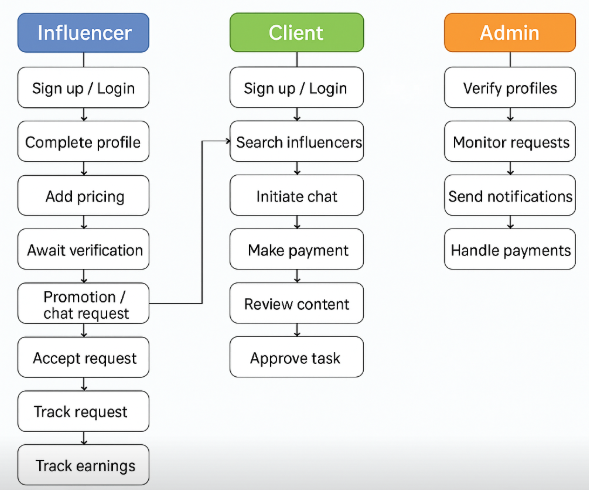
\includegraphics[height=0.5\textheight]{Chapters/Screenshot 2025-05-14 102150.png}
    \caption{System Workflow Diagram}
    \label{fig:system-workflow}
\end{figure}
  \end{justify}





\chapter{Literature Review}
\begin{justify}
    The growing prominence of influencer marketing, particularly in India, has opened new opportunities for digital engagement while also revealing significant structural and operational gaps. This chapter explores existing research, technological advancements, and real-world systems related to influencer-brand collaborations. It highlights their strengths, limitations, and how this project addresses current shortcomings.

    \section{Overview of Influencer Marketing}
    Influencer marketing is defined as a form of social media marketing that involves endorsements and product placements from individuals who have a dedicated social following and are viewed as experts within their niche. According to a 2023 report by Influencer Marketing Hub, influencer marketing grew into a \$21.1 billion global industry, with India showing one of the fastest growth rates due to a surge in smartphone usage and digital content consumption.
    \par
    Researchers have pointed out that influencer marketing works because it offers authentic, peer-driven engagement compared to traditional advertising. However, many academic and industry studies also acknowledge the lack of standardization and infrastructure in influencer-brand interactions.
    \section{Existing Platforms and Technologies}
    Several platforms such as Collabstr, Upfluence, Winkl, and Heepsy attempt to bridge the gap between influencers and brands. These platforms typically offer influencer search tools, campaign management, and analytics. However, most are either focused on Western markets or require paid subscriptions, which limits accessibility for Indian users.
Key limitations of these platforms include:
\begin{enumerate}
    \item 	Limited regional influencer coverage, particularly for Tier 2 and Tier 3 Indian cities.
    \item 	Lack of integrated real-time communication tools such as chat or collaborative workspaces.
    \item 	Delayed or insecure payment methods, which often lead to disputes or trust issues.
    \item 	Inadequate support for influencer-to-influencer collaborations and content co-creation.
\end{enumerate}
This project aims to overcome these challenges by tailoring the platform to the Indian market and integrating critical features such as secure payments, milestone tracking, and real-time chat.

\section{Payment and Escrow Systems in Digital Platforms}
Milestone-based payment systems, commonly used in freelancing platforms like Upwork and Freelancer, are proven to reduce fraud and increase transparency. They function by holding client payments in escrow and releasing funds upon task completion. Academic studies have shown that escrow-based models improve trust and transactional security in peer-to-peer marketplaces.
\par
However, such models are rarely seen in influencer platforms. This project integrates a milestone-based escrow system using Razorpay or Stripe, ensuring timely and fair payments and reducing disputes.
\section{Real-Time Communication and Collaboration Tools}
Effective communication is a key driver of successful collaborations. Platforms like Slack and Microsoft Teams offer real-time collaboration but are not optimized for influencer-brand dynamics. In the influencer marketing context, real-time chat helps in finalizing campaign details, clearing doubts, sharing briefs, and delivering feedback efficiently.
\par
By using Firebase Realtime Database, this platform supports instant messaging between clients and influencers, eliminating the dependence on external tools like emails or DMs, which are often unstructured and difficult to track.

\section{Verification Systems and Trust Building}
According to several research articles and industry whitepapers, trust is a major factor influencing digital collaborations. Fake profiles, bot-driven engagement, and unverifiable credentials reduce the effectiveness of influencer campaigns. Leading platforms like Instagram and Twitter offer blue tick verification, but they do not verify engagement authenticity.\par
This project incorporates a manual and automated influencer verification process, where influencers are required to submit identity documents, social handles, and engagement stats. The goal is to create a trustworthy ecosystem for brands to confidently engage with genuine creators.
\section{Co-Creation and Influencer Networks}
The literature also highlights the benefits of co-creation in influencer marketing. According to a 2021 study published in the Journal of Interactive Marketing, influencer collaboration leads to higher engagement rates and better content performance. However, most existing platforms ignore peer-to-peer features.
\par
Our project addresses this by offering influencer-to-influencer collaboration tools, enabling creators to pitch ideas, run joint campaigns, and grow their audience organically.

\section{Gaps in Existing Systems}


\begin{table}[h!]
\centering
\caption{Comparison of Features: Existing Platforms vs. Proposed Solution}
\begin{tabularx}{\textwidth}{>{\bfseries}l X X}
\toprule
Feature & Existing Platforms & Proposed Solution in Our Project \\
\midrule
Real-time chat & Rare or absent & Included via Firebase \\
Secure milestone payments & Rare & Integrated with Razorpay/Stripe escrow \\
Indian influencer focus & Limited & Fully India-specific platform \\
Verified influencer onboarding & Basic or absent & Manual + automated multi-step verification \\
Influencer collaboration tools & Not offered & Enabled through peer networking features \\
\bottomrule
\end{tabularx}
\end{table}


\end{justify}
\chapter{Proposed System}
\begin{justify}
    
\section{System Architecture}
The proposed system, Influencify, is a web-based platform designed to connect verified Indian influencers with brands, providing a secure, centralized environment for collaborations. It addresses key challenges in the current influencer marketing ecosystem, including transparency, secure payments, task tracking, and seamless communication. The system is highly scalable, modular, and user-friendly, enabling efficient management of influencer collaborations for both small and large-scale campaigns. The architecture is designed to support high performance, real-time interactions, and secure transactions, ensuring a smooth user experience.
The architecture of Influencify is composed of the following core components:
\begin{itemize}
    \item \textbf{Profile and Pricing Management:} Allows influencers to set pricing for different types of promotions (e.g., story posts, image uploads, video content) and manage their portfolios.
    
    \item \textbf{Search and Discovery Engine:} Enables brands to search for influencers based on filters like platform, follower count, engagement rate, and pricing, facilitating more targeted campaign planning.
    
    \item \textbf{Real-time Communication:} Powered by Firebase for instant chat functionality, ensuring timely responses and reducing communication gaps between influencers and clients.
    
    \item \textbf{Payment Processing Module:} Integrated with Razorpay or Stripe for secure, milestone-based escrow payments, ensuring fair transactions and protecting both parties.
    
    \item \textbf{Task Management and Tracking:} Provides tools for brands to send collaboration requests, track task progress, and confirm task completion before releasing payments.
    
    \item \textbf{Admin Panel:} Allows platform administrators to verify users, manage disputes, monitor transactions, and ensure platform security.
    
    \item \textbf{Analytics and Reporting:} Collects and analyzes data on influencer performance, campaign outcomes, and payment history to provide valuable insights to users.
\end{itemize}
\begin{figure}[H]
    \centering
    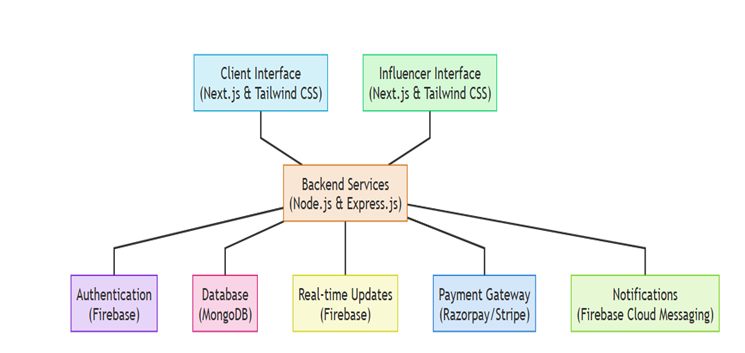
\includegraphics[height=0.3\textheight]{Chapters/Screenshot 2025-05-18 194104.png}
    \caption{System Architecture }
    \label{fig:system-workflow}
\end{figure}
\section{Features}
\subsection{Influencer Side Features}
\begin{enumerate}
    \item \textbf{Profile Creation & Management:} Influencers can create a comprehensive profile including personal information, social media links, niche, follower demographics, and engagement rates. They can update their profiles anytime to keep information current.
    \item \textbf{Pricing Setup:} Influencers set transparent prices for different promotion types such as story uploads, image posts, and video posts. Pricing can vary by platform (Instagram, YouTube, Facebook, etc.) and content type, allowing flexibility.
    \item	\textbf{Platform Selection:} Influencers specify on which platforms they want to offer promotions, helping clients filter based on campaign requirements.
    \item 	\textbf{Chat Requests:} Influencers receive and manage incoming chat requests from potential clients. The chat system supports real-time messaging to discuss campaign details efficiently.
    \item \textbf{Request Management:} Influencers can accept or reject promotion requests based on availability, campaign relevance, or other criteria.
    \item \textbf{Earnings & Payment History:} A detailed dashboard displays earnings, pending payments, transaction history, and milestone payments, providing full transparency.
    \item 	\textbf{Influencer-to-Influencer Collaboration:} Enables co-creation opportunities where influencers can collaborate on campaigns, share audiences, and increase organic reach.
\end{enumerate}
\subsection{Client Side Features}
\begin{enumerate}
    \item \textbf{Influencer Search & Filtering:} Clients can search influencers using filters like niche, platform, follower count, engagement rate, and pricing to find the best fit for their campaign.
    \item 	\textbf{Profile & Package Viewing:} Clients can view detailed influencer profiles, including previous work, reviews, and promotional packages.
    \item 	\textbf{Direct Chat:} Secure and real-time messaging with influencers to discuss campaign specifics, timelines, and deliverables.
    \item 	\textbf{Promotion Requests:} Clients can send promotion requests to influencers, outlining the campaign details and expectations.
    \item 	\textbf{Secure Payment System:} Payments are made securely through milestone-based escrow. Funds are held until campaign deliverables are approved.
    \item 	\textbf{Task Approval:} Clients review completed promotion posts and approve or dispute the work before payment is released.
\end{enumerate}
\subsection{Admin Side Features}
\begin{enumerate}
    \item 	\textbf{User Verification:} Admins verify authenticity of both influencers and clients through document checks, social media audits, and activity monitoring to maintain platform trust.
    \item 	\textbf{Monitoring & Moderation:} Admins monitor chats and promotion requests for policy compliance and fraud prevention.
    \item 	\textbf{Payment Tracking:} Oversees all payment transactions including escrow management, payment releases, refunds, and disputes.
    \item 	\textbf{Dispute Resolution:} Admins intervene in case of payment or content disputes, providing fair resolutions to maintain platform integrity.
    \item 	\textbf{Notification Management:} Admins can send targeted notifications and alerts to users about campaign updates, policy changes, or platform news.
\end{enumerate}
\section{Workflow}
\begin{enumerate}
\item \textbf{	Influencer Registration & Profile Creation: }Influencers sign up and complete their profile, including pricing and platform preferences.
\item 	\textbf{Client Browsing & Searching:} Clients search for influencers based on campaign needs using filters.
\item 	\textbf{Sending Promotion Requests:} Clients send detailed promotion requests to selected influencers.
\item 	\textbf{Influencer Response:} Influencers review requests and either accept or reject them.
\item 	\textbf{Payment Process Initiation:} Upon acceptance, clients make payment to the platform’s escrow system.
\item 	\textbf{Content Creation & Posting:} Influencers complete the promotional task by posting the agreed content on their platform(s).
\item 	\textbf{Client Approval:} Clients verify the content and approve or request modifications.
\item 	\textbf{Payment Release:} After client approval, funds are released from escrow to the influencer within 7 days.
\item \textbf{	Post-Campaign Review & Rating:} Both parties can rate and review each other to build platform credibility.
\end{enumerate}
\begin{figure}[H]
    \centering
    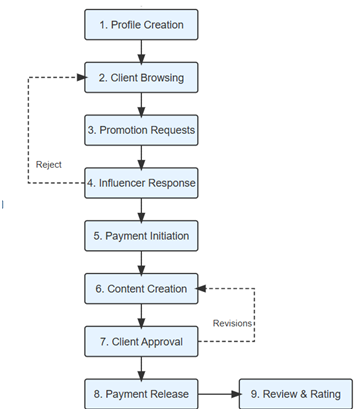
\includegraphics[height=0.4\textheight]{Chapters/Screenshot 2025-05-18 193856.png}
    \caption{Workflow of the System}
    \label{fig:system-workflow}
\end{figure}
\section{Components}
\subsection{Frontend:}
\begin{enumerate}
    \item Built with Next.js for server-side rendering and static generation, improving SEO and performance.
    \item Uses Tailwind CSS and CSS Modules for modular, responsive, and maintainable styling.
    \item Handles user interactions, profile management, search, chat UI, and payment interfaces.
\end{enumerate}
\subsection{Backend:}
\begin{enumerate}
    \item 	Developed with Node.js and Express.js to provide RESTful API endpoints.
    \item 	Manages authentication, business logic, campaign management, payment processing, and real-time notifications.
    \item 	Integrates with external services for payments and messaging.
\end{enumerate}
\subsection{Database:}
\begin{enumerate}
    \item MongoDB stores user data, campaign details, chat logs, and transaction records in flexible JSON-like documents.
    \item Ensures fast querying, indexing, and scalability for growing user base.
\end{enumerate}
\subsection{Real-Time Communication:}
\begin{enumerate}
    \item 	Uses Firebase Realtime Database for instant chat message synchronization across devices.
    \item 	Supports offline persistence and automatic sync when connectivity is restored.
\end{enumerate}
\subsection{Authentication:}
\begin{enumerate}
    \item Employs Firebase Authentication supporting Google Sign-In and email/password login.
    \item 	Ensures secure session management and role-based access control.
\end{enumerate}
\subsection{Payment System:}
\begin{enumerate}
    \item Integrates Razorpay and Stripe to process secure milestone-based escrow payments.
    \item	Manages payment releases, refunds, multi-currency support, and transaction tracking.
\end{enumerate}
notifications for chats, campaign updates, payments, and alerts.
    \begin{figure}[H]
    \centering
    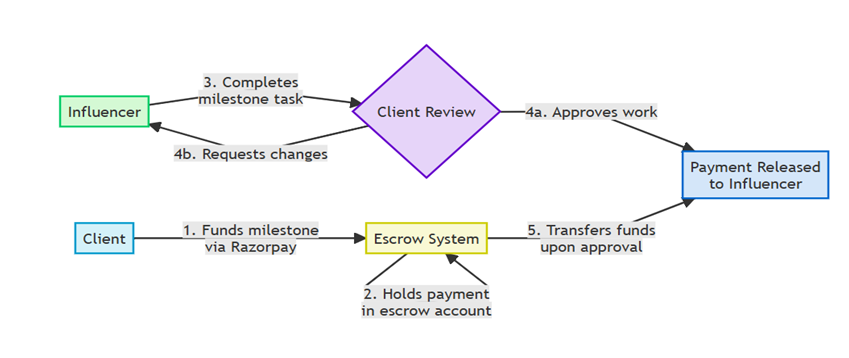
\includegraphics[height=0.3\textheight]{Chapters/Screenshot 2025-05-18 194646.png}
    \caption{Escrow Payment Flow}
    \label{fig:system-workflow}
\end{figure}
\subsection{	Notification System:}
	Uses Firebase Cloud Messaging (FCM) to send real-time push 
\section{Limitations of Existing Solutions}

\begin{itemize}
    \item \textbf{Lack of Trust and Verification:}
    Many influencer platforms do not verify the credibility of influencers or brands, which can result in fraud, fake profiles, or unreliable partnerships.
    Influencify provides a verified platform where both influencers and clients go through a rigorous verification process. Influencers can showcase their real social media metrics and profiles, ensuring that both parties can trust each other’s legitimacy.
    
    \item \textbf{Fragmented Communication:}
    Influencers and brands often communicate via informal channels like social media DMs, leading to miscommunication, delays, or misunderstandings. There’s no centralized record of conversations.
    Influencify integrates in-app chat functionality using Firebase Realtime Database, which allows clients and influencers to directly communicate within the platform. All conversations are logged, ensuring that there’s a clear, transparent record of discussions and agreements.

    \item \textbf{Unreliable Payment Systems:}
    Influencers face delayed or inconsistent payments after completing promotional tasks, and platforms often lack a secure and transparent payment process.
    Influencify uses a secure escrow payment system through integrated payment gateways like Razorpay or Stripe. The payment is held in escrow until the influencer completes the task, and only when the client confirms the work, is the payment released to the influencer. This ensures fair and timely transactions for both parties.

    \item \textbf{Limited Customization for Clients:}
    Existing platforms may not offer the right tools for clients to filter and find influencers who match their specific needs, or to customize promotion packages.
    Clients on Influencify can search and filter influencers based on multiple parameters such as category, platform, followers, price range, and more. Additionally, clients can send customized promotion requests based on specific requirements, ensuring a better match between the brand and influencer.

    \item \textbf{Absence of Task Tracking and Milestones:}
    Many platforms fail to provide a structured system for task tracking, leading to confusion about deliverables and timelines.
    Influencify introduces a milestone-based system where each task is tracked from creation to completion. Influencers and clients both know what’s expected, and payments are only processed after the client confirms the deliverables. This reduces ambiguity and ensures smoother workflows.

    \item \textbf{Inefficient Dispute Resolution:}
    In case of issues or disagreements, many platforms offer minimal dispute resolution support, leaving users to handle conflicts without clear processes.
    Influenciy includes a dispute resolution system where the admin team can intervene if any issues arise between influencers and clients. This ensures that both parties have a neutral, fair process to address conflicts and concerns.

    \item \textbf{No Collaboration Opportunities:}
    Many platforms don’t encourage collaboration between influencers, missing the potential for co-created campaigns and organic growth.
    Influencify promotes influencer-to-influencer collaborations, where influencers can connect with each other to collaborate on campaigns, exchange ideas, and co-create content. This not only benefits influencers but also fosters organic growth and cross-promotion.
\end{itemize}
\end{justify}

\chapter{Technologies Used}
\begin{justify}
    
\section{Front-end Technologies}
\subsection{Next.js} \\
Next.js is a powerful React framework that enables developers to build modern, high-performance web applications with server-side rendering (SSR) and static site generation (SSG). These features are essential for building fast, SEO-friendly, and scalable platforms like NFLUENCIFY. Key features include:
\begin{itemize}
    \item Server-Side Rendering (SSR): Renders pages on the server before sending them to the client, reducing initial load time and improving SEO.
    \item 	Static Site Generation (SSG): Pre-generates pages at build time for lightning-fast loading and reduced server load.
    \item 	Dynamic Routing: Supports both file-based routing and dynamic routes for flexible, intuitive navigation structures.
    \item 	API Routes: Allows seamless serverless API creation, eliminating the need for a separate backend for many use cases.
    \item 	Image Optimization: Automatic image optimization to improve loading speed and performance.
    \item 	Built-in CSS and Sass Support: Simplifies styling with support for CSS Modules, global styles, and Sass.
    \item 	Internationalization: Out-of-the-box support for multi-language applications.
    \item 	Incremental Static Regeneration (ISR): Enables real-time content updates without full rebuilds, perfect for live influencer profiles.
\end{itemize}
Next.js is ideal for NFLUENCIFY as it provides the speed, scalability, and SEO optimization needed to handle high traffic and dynamic content, ensuring a seamless experience for both influencers and brands.
\par

\subsection{CSS Modules / Tailwind CSS} 
CSS Modules ensure style encapsulation by scoping CSS to specific components, which prevents style conflicts and enhances maintainability. Tailwind CSS, a utility-first CSS framework, is used to rapidly build custom designs with consistent spacing, colors, and responsiveness. The combination of these tools helps maintain a clean and scalable frontend design system.
\begin{itemize}
    \item 	Responsive Design: Built-in support for mobile-first design with responsive breakpoints.
    \item 	Utility-First Approach: Focuses on low-level utility classes like p-4, text-center, and bg-gray-200 for highly customized designs without writing complex CSS.
    \item 	Customization: Fully customizable via a configuration file, enabling brand-specific styling.
    \item 	Component Reusability: Encourages building reusable UI components, reducing code repetition and improving maintainability.
    \item 	Performance: Small file sizes and fast load times due to optimized, purged CSS for production builds.
    \end{itemize}

     CSS Modules provide scoped CSS to specific components, avoiding global conflicts and improving maintainability, making it easier to build complex, scalable UIs.


\section{Backend Technologies}
\begin{enumerate}
\item \textbf{Node.js with Express.js}\\
The backend of Influencify is built on Node.js, a high-performance JavaScript runtime, and Express.js, a minimalist web framework for Node. This stack provides the foundational structure for managing RESTful APIs, routing, user session management, authentication flows, business logic, and third-party integrations such as payments and messaging services.

\item\textbf{MongoDB}\\
MongoDB is a NoSQL document-oriented database that stores data in a flexible, JSON-like format. It is ideal for handling diverse data structures such as user profiles, collaboration requests, chat logs, and payment records. Its scalability and indexing capabilities make it well-suited for the growing data needs of the platform.
\end{enumerate}

\section{Real-Time Communication}
\textbf{Firebase Realtime Database}\\
To power instant and dynamic communication between influencers and clients, the platform employs Firebase Realtime Database—a cloud-hosted NoSQL solution that specializes in real-time data synchronization. This technology ensures that messages appear instantly across all connected devices, fostering fluid, uninterrupted conversations.
\par
What sets Firebase apart is its ability to push updates automatically, removing the need for users to refresh or reload pages. In addition, it offers offline persistence, meaning users can continue chatting even with intermittent connectivity—conversations are synced the moment the connection is restored.
\par
This technology forms the backbone of Influencify's live chat system, enabling responsive, real-time collaboration and building trust through timely interactions.
\section{User Authentication}
\textbf{Google Sign-In and Email/Password Authentication}\\
Influencify supports both social login (Google Sign-In) and traditional email/password login to provide flexible and secure authentication methods for users. Firebase Authentication simplifies the process by offering ready-to-use authentication UIs, robust session management, and integration with other Firebase services. Custom logic can also be implemented to handle role-based access control and user verification.
\section{Payment Integration}
The platform includes secure and reliable payment gateways—Razorpay and Stripe—to handle financial transactions. Payments from clients are initially directed to the platform's escrow account and are only released to the influencer once the client confirms campaign fulfillment. This two-step release process ensures trust and transparency. These gateways also support refund handling, payment status updates, and multi-currency transactions.

\section{ Notifications }
\textbf{Firebase Cloud Messaging }\\
Firebase Cloud Messaging is used to send real-time web push notifications to users for various events such as new chat messages, campaign updates, approval confirmations, and payment alerts. This keeps users actively informed even when they are not on the platform. FCM supports scheduling, priority messaging, and cross-platform delivery (web and mobile).


\end{justify}

\chapter{Innovations and Impact}
\begin{justify}
    \section{Conclusion}
    
The Influencify platform marks a transformative leap in the world of brand collaborations and influencer marketing, offering a comprehensive solution that combines cutting-edge technologies with user-centric features. Designed to address the unique challenges faced by both influencers and brands, Influencify enhances the process of connecting, negotiating, and executing successful marketing campaigns. By integrating powerful tools such as Razorpay and Stripe for payment processing, the platform ensures that all financial transactions are secure, transparent, and efficient. These payment gateways provide a seamless experience, supporting multi-currency transactions and refunds, which is especially valuable in a diverse market like India.

One of the standout features of Influencify is its two-step payment release system, which places an emphasis on trust and accountability. Payments are initially directed to an escrow account, and only released to the influencer once the client has confirmed that the campaign requirements have been met. This mechanism fosters a sense of security for both clients and influencers, reducing the risks associated with payment disputes and ensuring that all parties are satisfied with the outcome of a campaign before the financial transaction is completed. This added layer of security helps establish a more reliable and fair marketplace for influencer collaborations.

Furthermore, Influencify leverages Firebase Cloud Messaging (FCM) to keep users informed in real-time. Whether it is updates on campaign progress, new chat messages, approval confirmations, or payment alerts, FCM ensures that users are always up to date, even when they are not actively engaging with the platform. The ability to receive instant notifications helps maintain a continuous flow of communication and keeps users engaged throughout the lifecycle of a campaign. This feature enhances the overall user experience, creating a dynamic environment that facilitates timely responses and decision-making.

The integration of these technologies within Influencify is not only a testament to the platform’s commitment to providing a secure, efficient, and user-friendly environment but also underscores its role in modernizing the influencer marketing industry. By combining robust backend services with intuitive interfaces, Influencify reduces the complexity typically associated with influencer-brand collaborations, making it easier for users to navigate and maximize the potential of their partnerships. The platform’s streamlined workflow, combined with the security of trusted payment gateways and real-time notifications, ensures that users can focus on building meaningful relationships rather than being bogged down by administrative or transactional hurdles.

As Influencify continues to evolve, it is poised to become a pivotal player in the future of influencer marketing. The platform’s ability to combine the latest in payment technology, real-time communication, and cloud-based solutions provides a robust foundation for future growth. It holds the potential to set new standards for the influencer marketing industry, offering a scalable and adaptable solution that can meet the needs of a diverse and dynamic market. By reducing human error, increasing transparency, and fostering collaboration, Influencify is not only enhancing the influencer-brand relationship but is also shaping the future of digital marketing in an increasingly interconnected world.

Ultimately, Influencify is more than just a platform; it is an innovative tool that empowers both influencers and brands to navigate the complexities of digital marketing with ease and confidence. With its seamless payment systems, intuitive communication tools, and secure, scalable infrastructure, the platform stands as a benchmark for future developments in the influencer marketing space, driving efficiency, trust, and transparency in every aspect of the process.
\section{Future Directions}

As the Influencify platform continues to evolve, several promising directions for future development can significantly enhance the user experience, broaden its reach, and expand its capabilities. These enhancements aim to further streamline the influencer-brand collaboration process and offer more personalized, data-driven, and efficient tools for both influencers and clients.

\begin{itemize}
    \item \textbf{Mobile App Development} \\
    To make the platform even more accessible and convenient for users on the go, the development of mobile applications using React Native is a crucial next step. Mobile apps will provide users with the ability to manage their campaigns, communications, payments, and notifications from anywhere, ensuring that both influencers and clients can stay connected and engaged at all times. The app will bring the full functionality of Influencify to smartphones, improving user accessibility, convenience, and overall satisfaction.
    
    \item \textbf{AI-Based Influencer Suggestion System} \\
    Leveraging artificial intelligence to build a sophisticated influencer suggestion system can drastically improve the efficiency and relevance of influencer-brand matches. By analyzing past campaign data, audience demographics, engagement rates, and other metrics, AI can provide personalized recommendations for both influencers and brands. This AI-powered system will save time by suggesting the most suitable influencers based on campaign requirements, thus increasing the chances of successful partnerships and helping brands target the right audience more effectively.
    
    \item \textbf{Multi-Language Support} \\
    With the platform's increasing popularity, especially in diverse markets like India, adding multi-language support will be essential to reach a broader audience. Offering multiple language options will help break down language barriers and enable influencers and brands from different regions to use Influencify seamlessly. This feature will not only expand the platform's user base but also create a more inclusive experience for users who may feel more comfortable communicating in their native language.
    
    \item \textbf{Analytics Dashboard for Influencers and Clients} \\
    Data-driven decision-making is key to the success of any marketing campaign. To provide influencers and brands with better insights into their campaigns, an advanced analytics dashboard will be developed. This dashboard will present real-time data on engagement, audience demographics, performance metrics, ROI, and more, enabling both influencers and clients to optimize their strategies. Influencers will be able to track their campaign performance, audience engagement, and potential revenue, while brands will gain deeper insights into campaign effectiveness and ROI, allowing them to make informed decisions on future collaborations.
    
    \item \textbf{GST Invoicing and Compliance for Influencers} \\
    As India continues to evolve its tax policies, incorporating GST invoicing and compliance features into the platform will be crucial. Influencers will be able to generate automated GST-compliant invoices for their earnings, ensuring they meet legal requirements and reduce the chances of errors in tax filings. This feature will not only simplify the process for influencers but also foster trust with brands, as it ensures that all payments are compliant with tax regulations. The platform can also provide reminders and tools to help influencers stay up to date with changes in tax laws and compliance requirements.
\end{itemize}



\end{justify}

%\include{./Chapters/Chapter-7}
%\include{./Chapters/Chapter-8}
%\include{./Chapters/Chapter-9}
%\bibliographystyle{IEEEtran}
\begin{thebibliography}{99}
\bibitem{firebase2024}
Google, “Firebase Realtime Database Documentation,” 2024. [Online]. Available: \url{https://firebase.google.com/docs/database}. [Accessed: May 13, 2025].

\bibitem{firebaseBlog2023}
J. Lee, “Optimizing Mobile Apps with Firebase Realtime Database,” Firebase Blog, 2023. [Online]. Available: \url{https://firebase.googleblog.com/2023/05/realtime-database-performance.html}. [Accessed: May 13, 2025].

\bibitem{stripeDocs}
Stripe, “Stripe API Documentation,” 2025. [Online]. Available: \url{https://stripe.com/docs/api}. [Accessed: May 13, 2025].

\bibitem{kumar2021}
A. Kumar and R. Sharma, The Role of Technology in Influencer Marketing Platforms, Tech Innovations Press, 2021.

\bibitem{patel2022}
M. Patel, “Building Secure Payment Systems for E-Commerce,” Financial Tech Review, 2022. [Online]. Available: \url{https://www.examplelink.com/securepayments}. [Accessed: May 13, 2025].

\bibitem{davis2021}
R. Davis, “Ensuring Safe and Verified Transactions in Digital Platforms,” Cybersecurity Insights, 2021. [Online]. Available: \url{https://www.examplelink.com/verificationmethods}. [Accessed: May 13, 2025].

\bibitem{gupta2019}
P. Gupta, “Building Scalable Web Applications with Node.js and Express,” Web Dev Journal, 2019. [Online]. Available: \url{https://www.examplelink.com/nodejsweb}. [Accessed: May 13, 2025].

\bibitem{sharma2021}
S. Sharma, “Optimizing Payment Gateways: A Case Study on Razorpay and Stripe,” E-Commerce Solutions, 2021. [Accessed: May 13, 2025].

\end{thebibliography}

\addcontentsline{toc}{chapter}{References}
\end{document}